\documentclass[tikz,border=2pt]{standalone}
% ---------------------------------------------------------------------------
% figures/house.tex -- the shared look. Every figure \input's this, so six
% figures look like one hand drew them instead of six.
%
% HOW FIGURES WORK HERE. tikz/pgf is NOT on ACM's production package list, so
% the documents never load it. Each figure is its own standalone document in
% this directory, compiled to a PDF by `make figures`, and pulled into a
% section with
%
%     \begin{figure}
%       \centering
%       \includegraphics{figures/my-figure}
%       \caption{What to LOOK at, not what the figure is of.}
%       \label{fig:my-figure}
%     \end{figure}
%
% Three conventions:
%   * a float sits where it is discussed;
%   * a caption says what to look at, not what the figure is of;
%   * a figure is checked by rendering it and looking, not by a clean compile.
%
% The palette below is the same as the one in preamble.tex. It is repeated
% rather than shared because these are standalone documents that never see the
% paper's preamble, so a colour changed there must be changed here too.
% ---------------------------------------------------------------------------
\usepackage{amsmath}
% The figures build with LuaLaTeX like the documents, so their text is the
% paper's Libertine and their code is the paper's Iosevka.
\usepackage{fontspec}
\setmainfont{LinLibertine_R.otf}[BoldFont=LinLibertine_RB.otf,ItalicFont=LinLibertine_RI.otf,BoldItalicFont=LinLibertine_RBI.otf,Ligatures=TeX]
\setmonofont{Iosevka Custom}[Scale=MatchLowercase,RawFeature={-liga,-calt,-clig,-dlig}]
% Math in the figures is the paper's math: acmart sets Libertinus Math under
% LuaTeX, so the letters on a wire match the letters in the text around it.
\usepackage{unicode-math}
\setmathfont{LibertinusMath-Regular.otf}
\usetikzlibrary{positioning,arrows.meta,fit,backgrounds,calc}

% Blackboard Z, which the documents get from the paper preamble.
% Kept here so a figure never reaches for the paper's preamble.
\newcommand{\Z}{\mathbb{Z}}


\definecolor{ink}{HTML}{16191D}
\definecolor{accent}{HTML}{1F4E79}
\definecolor{accentsoft}{HTML}{E8EEF4}
% accent, accentwarm and accentplum mark the temporary's basis level -- level
% 0, 1, 2 -- wherever a picture or a matrix has to show which branch is which.
\definecolor{accentwarm}{HTML}{9A5B00}
\definecolor{accentplum}{HTML}{8E2F5F}
\definecolor{muted}{HTML}{5B6470}
\definecolor{hairline}{HTML}{C9CFD6}

\tikzset{
  % Every figure inherits this: thin lines, small type, generous air.
  house/.style={
    >={Stealth[length=2.1mm, width=1.6mm]},
    line width=0.5pt,
    node distance=9mm and 15mm,
    every node/.style={font=\small},
  },
  % A thing.
  box/.style={
    draw=ink, line width=0.5pt, rounded corners=1.5pt,
    inner xsep=6pt, inner ysep=4pt, align=center,
  },
  % A thing we are drawing attention to. One per figure, at most.
  boxhi/.style={box, draw=accent, fill=accentsoft, text=ink},
  % A thing that is context, not content.
  boxdim/.style={box, draw=hairline, text=muted},
  % An arrow, and the word on it.
  flow/.style={->, draw=ink},
  flowdim/.style={->, draw=hairline},
  lbl/.style={font=\footnotesize\itshape, text=accent, inner sep=2pt},
  lbldim/.style={font=\footnotesize, text=muted, inner sep=2pt},
  % A dashed grouping rectangle behind a set of nodes.
  group/.style={draw=hairline, dashed, rounded corners=2pt, inner sep=7pt},
}

\begin{document}
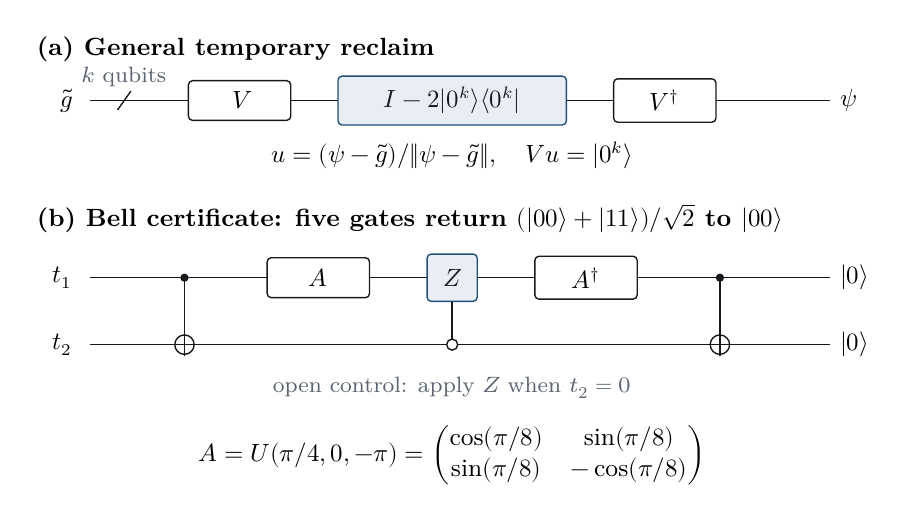
\begin{tikzpicture}[house]
\node[anchor=west,font=\small\bfseries] at (0,.65) {(a) General temporary reclaim};
\node[anchor=east] at (.7,0) {$\tilde g$};
\draw[ink] (.8,0)--(10.2,0);
\draw[ink] (1.15,-.12)--(1.32,.12);
\node[lbldim,above] at (1.23,.1) {$k$ qubits};
\node[box,fill=white,minimum width=13mm] at (2.7,0) {$V$};
\node[boxhi,minimum width=29mm] at (5.4,0) {$I-2|0^k\rangle\langle0^k|$};
\node[box,fill=white,minimum width=13mm] at (8.1,0) {$V^{\dagger}$};
\node[anchor=west] at (10.2,0) {$\psi$};
\node[align=center] at (5.4,-.7) {$u=(\psi-\tilde g)/\|\psi-\tilde g\|,\quad Vu=|0^k\rangle$};
\node[anchor=west,font=\small\bfseries] at (0,-1.5) {(b) Bell certificate: five gates return $(|00\rangle+|11\rangle)/\sqrt2$ to $|00\rangle$};
\foreach \y/\name in {-2.25/t_1,-3.1/t_2} {
 \node[anchor=east] at (.7,\y) {$\name$};
 \draw[ink] (.8,\y)--(10.2,\y);
 \node[anchor=west] at (10.2,\y) {$|0\rangle$};
}
\foreach \x in {2,8.8} {
 \draw[ink] (\x,-2.25)--(\x,-3.1);
 \fill[ink] (\x,-2.25) circle (1.5pt);
 \draw[ink,fill=white] (\x,-3.1) circle (3.5pt);
 \draw[ink] (\x,-3.25)--(\x,-2.95);
 \draw[ink] (\x-.15,-3.1)--(\x+.15,-3.1);
}
\node[box,fill=white,minimum width=13mm] at (3.7,-2.25) {$A$};
\draw[ink] (5.4,-2.25)--(5.4,-3.1);
\node[boxhi,minimum size=6mm] at (5.4,-2.25) {$Z$};
\draw[ink,fill=white] (5.4,-3.1) circle (2pt);
\node[box,fill=white,minimum width=13mm] at (7.1,-2.25) {$A^{\dagger}$};
\node[lbldim] at (5.4,-3.65) {open control: apply $Z$ when $t_2=0$};
\node at (5.4,-4.5) {$A=U(\pi/4,0,-\pi)=\begin{pmatrix}\cos(\pi/8)&\sin(\pi/8)\\\sin(\pi/8)&-\cos(\pi/8)\end{pmatrix}$};
\end{tikzpicture}
\end{document}
